\chapter*{Outlier / Anomaly detection}

In statistics, an outlier is an observation point that is distant from other observations. For this reason we apply outlier / anomaly detection for each class of our dataset in order to consider which data for each class could be excluded from the data set.
Below is shown an example of outlier detection applied to the subset that correspond to the letter `A'.
We calculate for all the samples the leave-one-out Gaussian Kernel density, KNN density, KNN average relative density and distance to K-th nearest neighbor for with K=5.\\
For each of the metrics, we sort the outlier scores and inspect their distribution. We set an outlier threshold where there is a significant ``jump'' in the scores, in order to have around 35 outliers (about 5\% of the total samples). We consider only the outliers which are detected by all four methods, and in this way we obtain 4 outliers (about 0.5\% of the samples).
In the bottom table are specified our results:
\begin{center}
    \begin{tabular}{ | p{3cm} | p{9cm} |}
    \hline
    \textbf{Method}  & \textbf{Selected outliers (indices)} \\
    \hline
    Gaussian Kernel density & [
   495
   741
   311
   133
   159
    51
    18
   399
    86
   739
   136
   566
   515
   423
     2
   227
   760
   285
   489
   152
   149
   572
   655
   688
   469
   114
   124
   762
   130
   638
   327
   645
   307 ]\\
    \hline
    KNN density & [ 18
   311
   495
   741
   133
   159
   515
    86
   399
    51
   739
   136
   489
   566
   285
   116
   688
   760
   227
   152
   423
   500
   469
   114
   655
     2
   149
   657
   504
   696
   238
   604
   572
   439
   124 ] \\
    \hline
    KNN average relative density & [ 197
   156
   102
   215
   356
    31
   399
   217
   127
   573
   701
   617
   124
   355
   530
    86
    36
   304
   450
   184
   133
   452
   321
   183
   746
   728
   714
   724
   638
   627
   285
   149 ]\\
    \hline
    Distance to 5th nearest neighbor & [     18
   311
   116
   515
   741
   399
   439
   500
    86
   133
   230
   495
   739
   159
   292
   489
   657
    51
   132
   136
   152
   238
   284
   285
   390
   438
   604
   688
    57
   114
   212
   227
   504
   566
   655
   696 ]\\
    \hline
    Common to all method & [ 51    86   739   688 ]\\
    \hline
    \end{tabular}
\end{center}

In figure  \ref{fig:r1} we represent one bar plot for each metrics. Each column is a pattern and the y-axis is the outlier score density (or distance for for 5th nearest neighbor ).  Red columns are patterns with lower outlier score (or highest for 5th nearest neighbor) that we decided to set as otliers.

\begin{figure}[htbp]
        \center
       	\begin{subfigure}[b]{0.46\textwidth}
                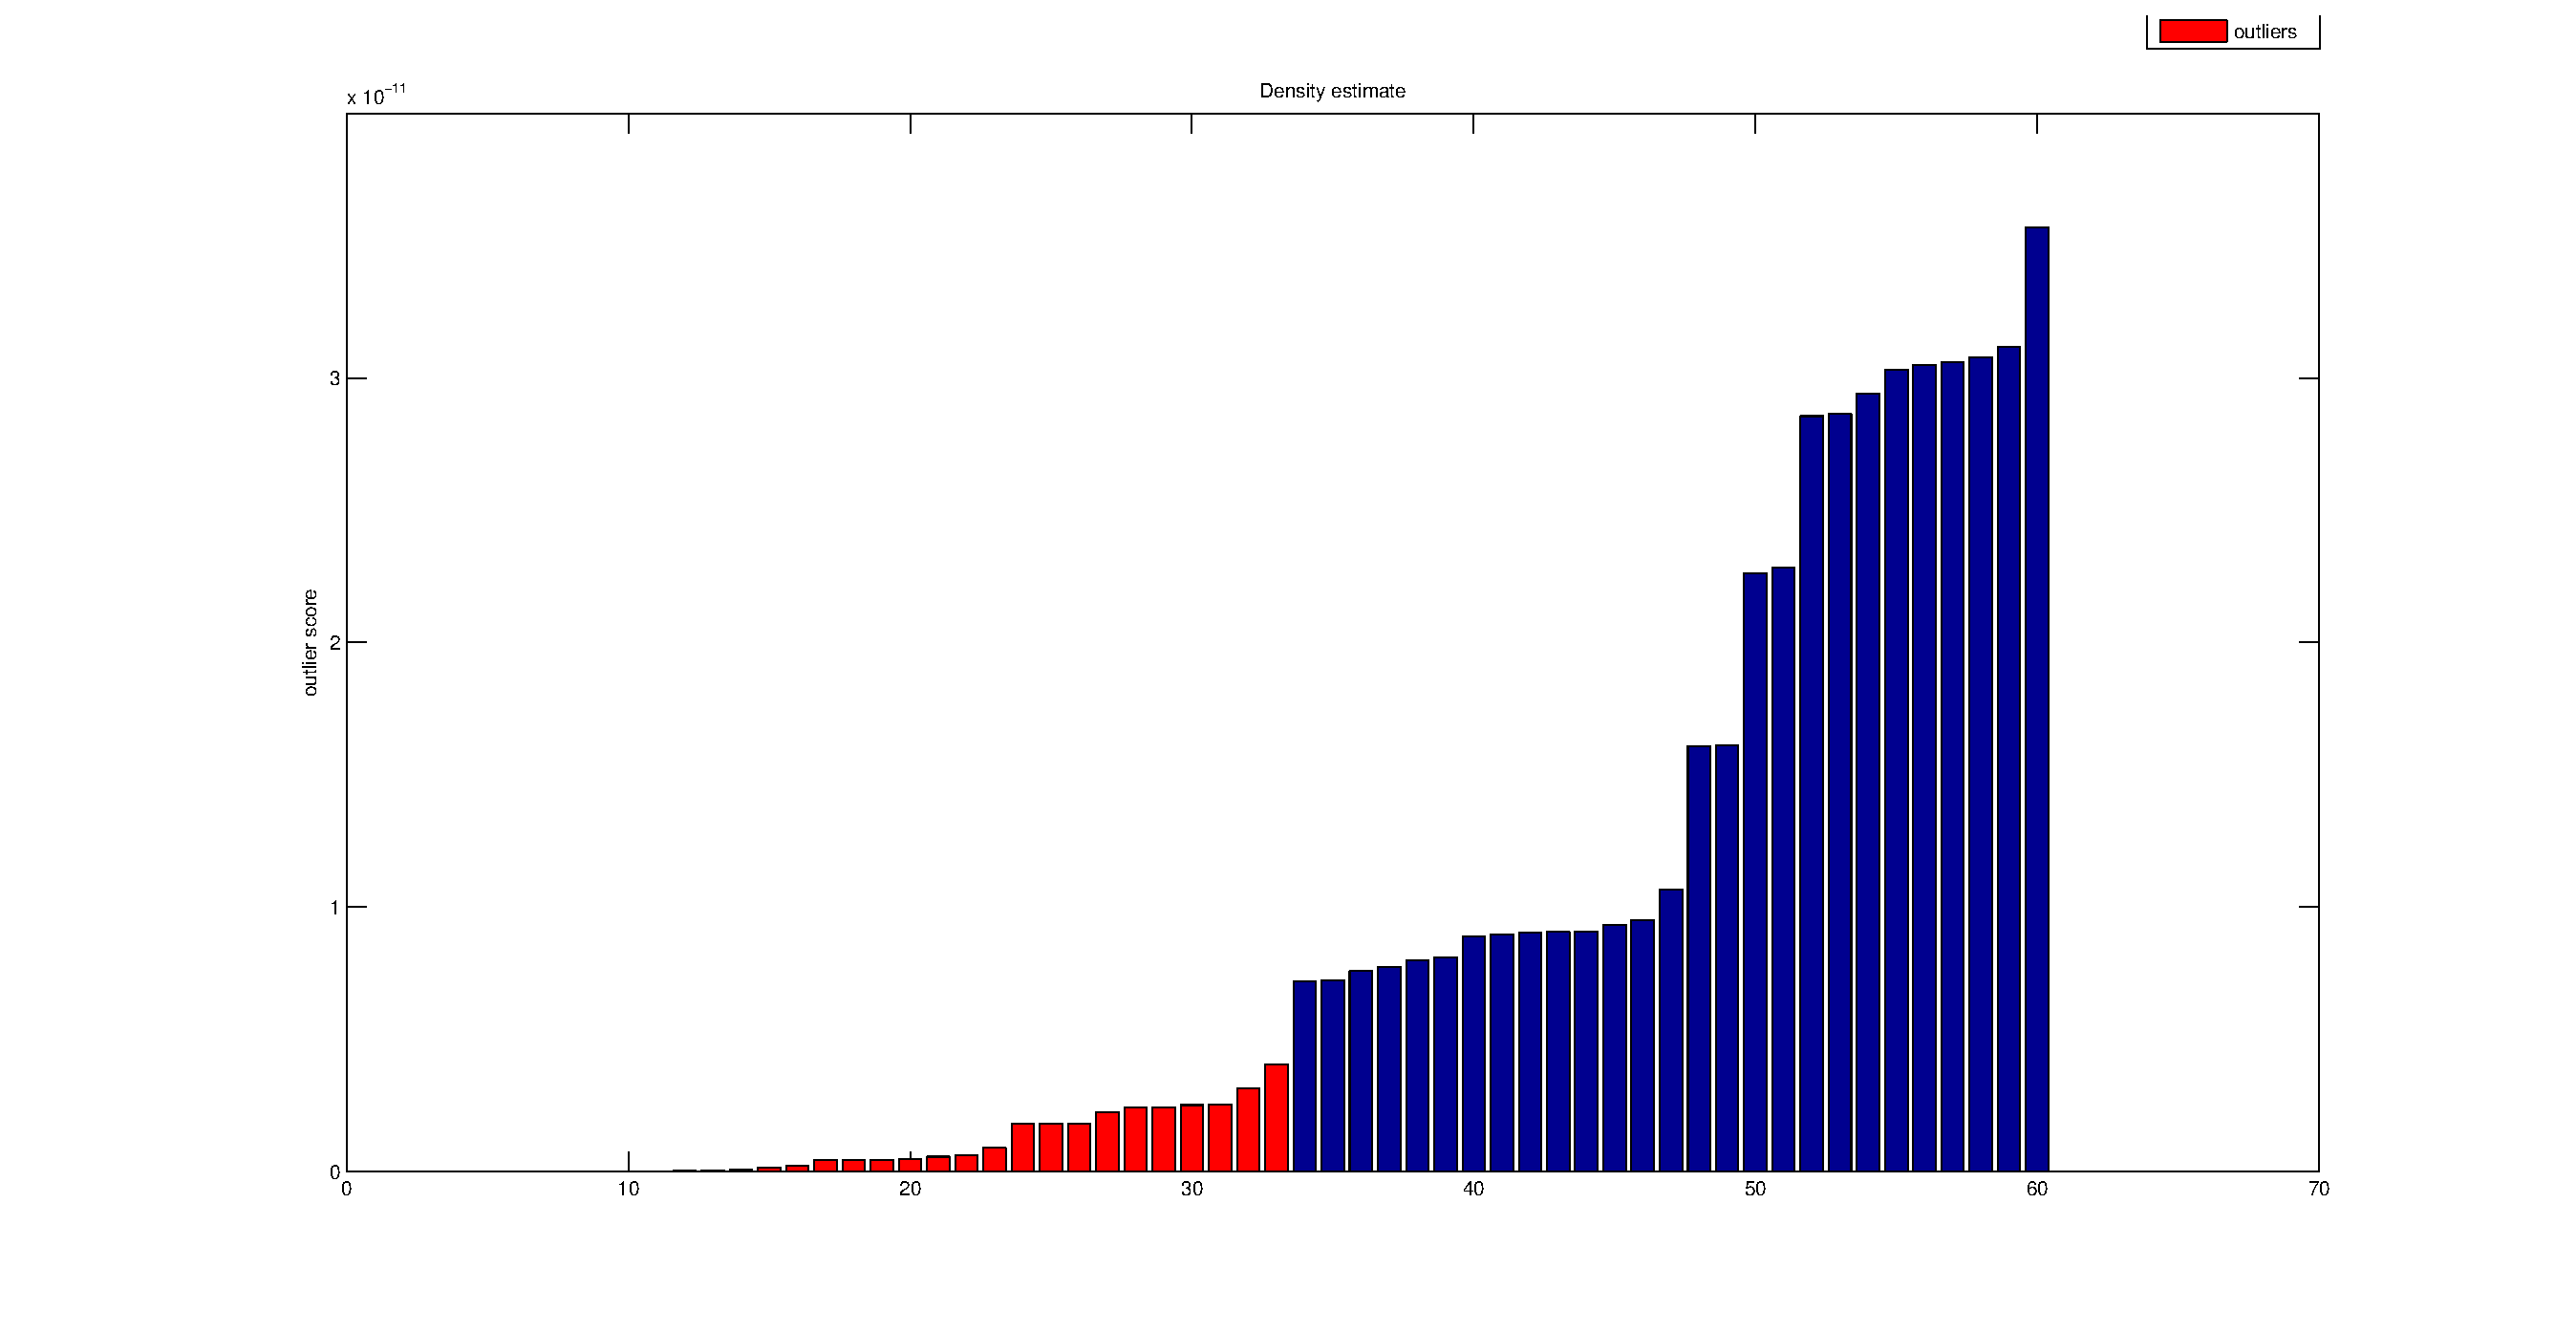
\includegraphics[width=7.4cm]{figures/01.eps}
                \caption{Density estimate outliers}
        \end{subfigure}%
        \qquad
        \begin{subfigure}[b]{0.46\textwidth}
                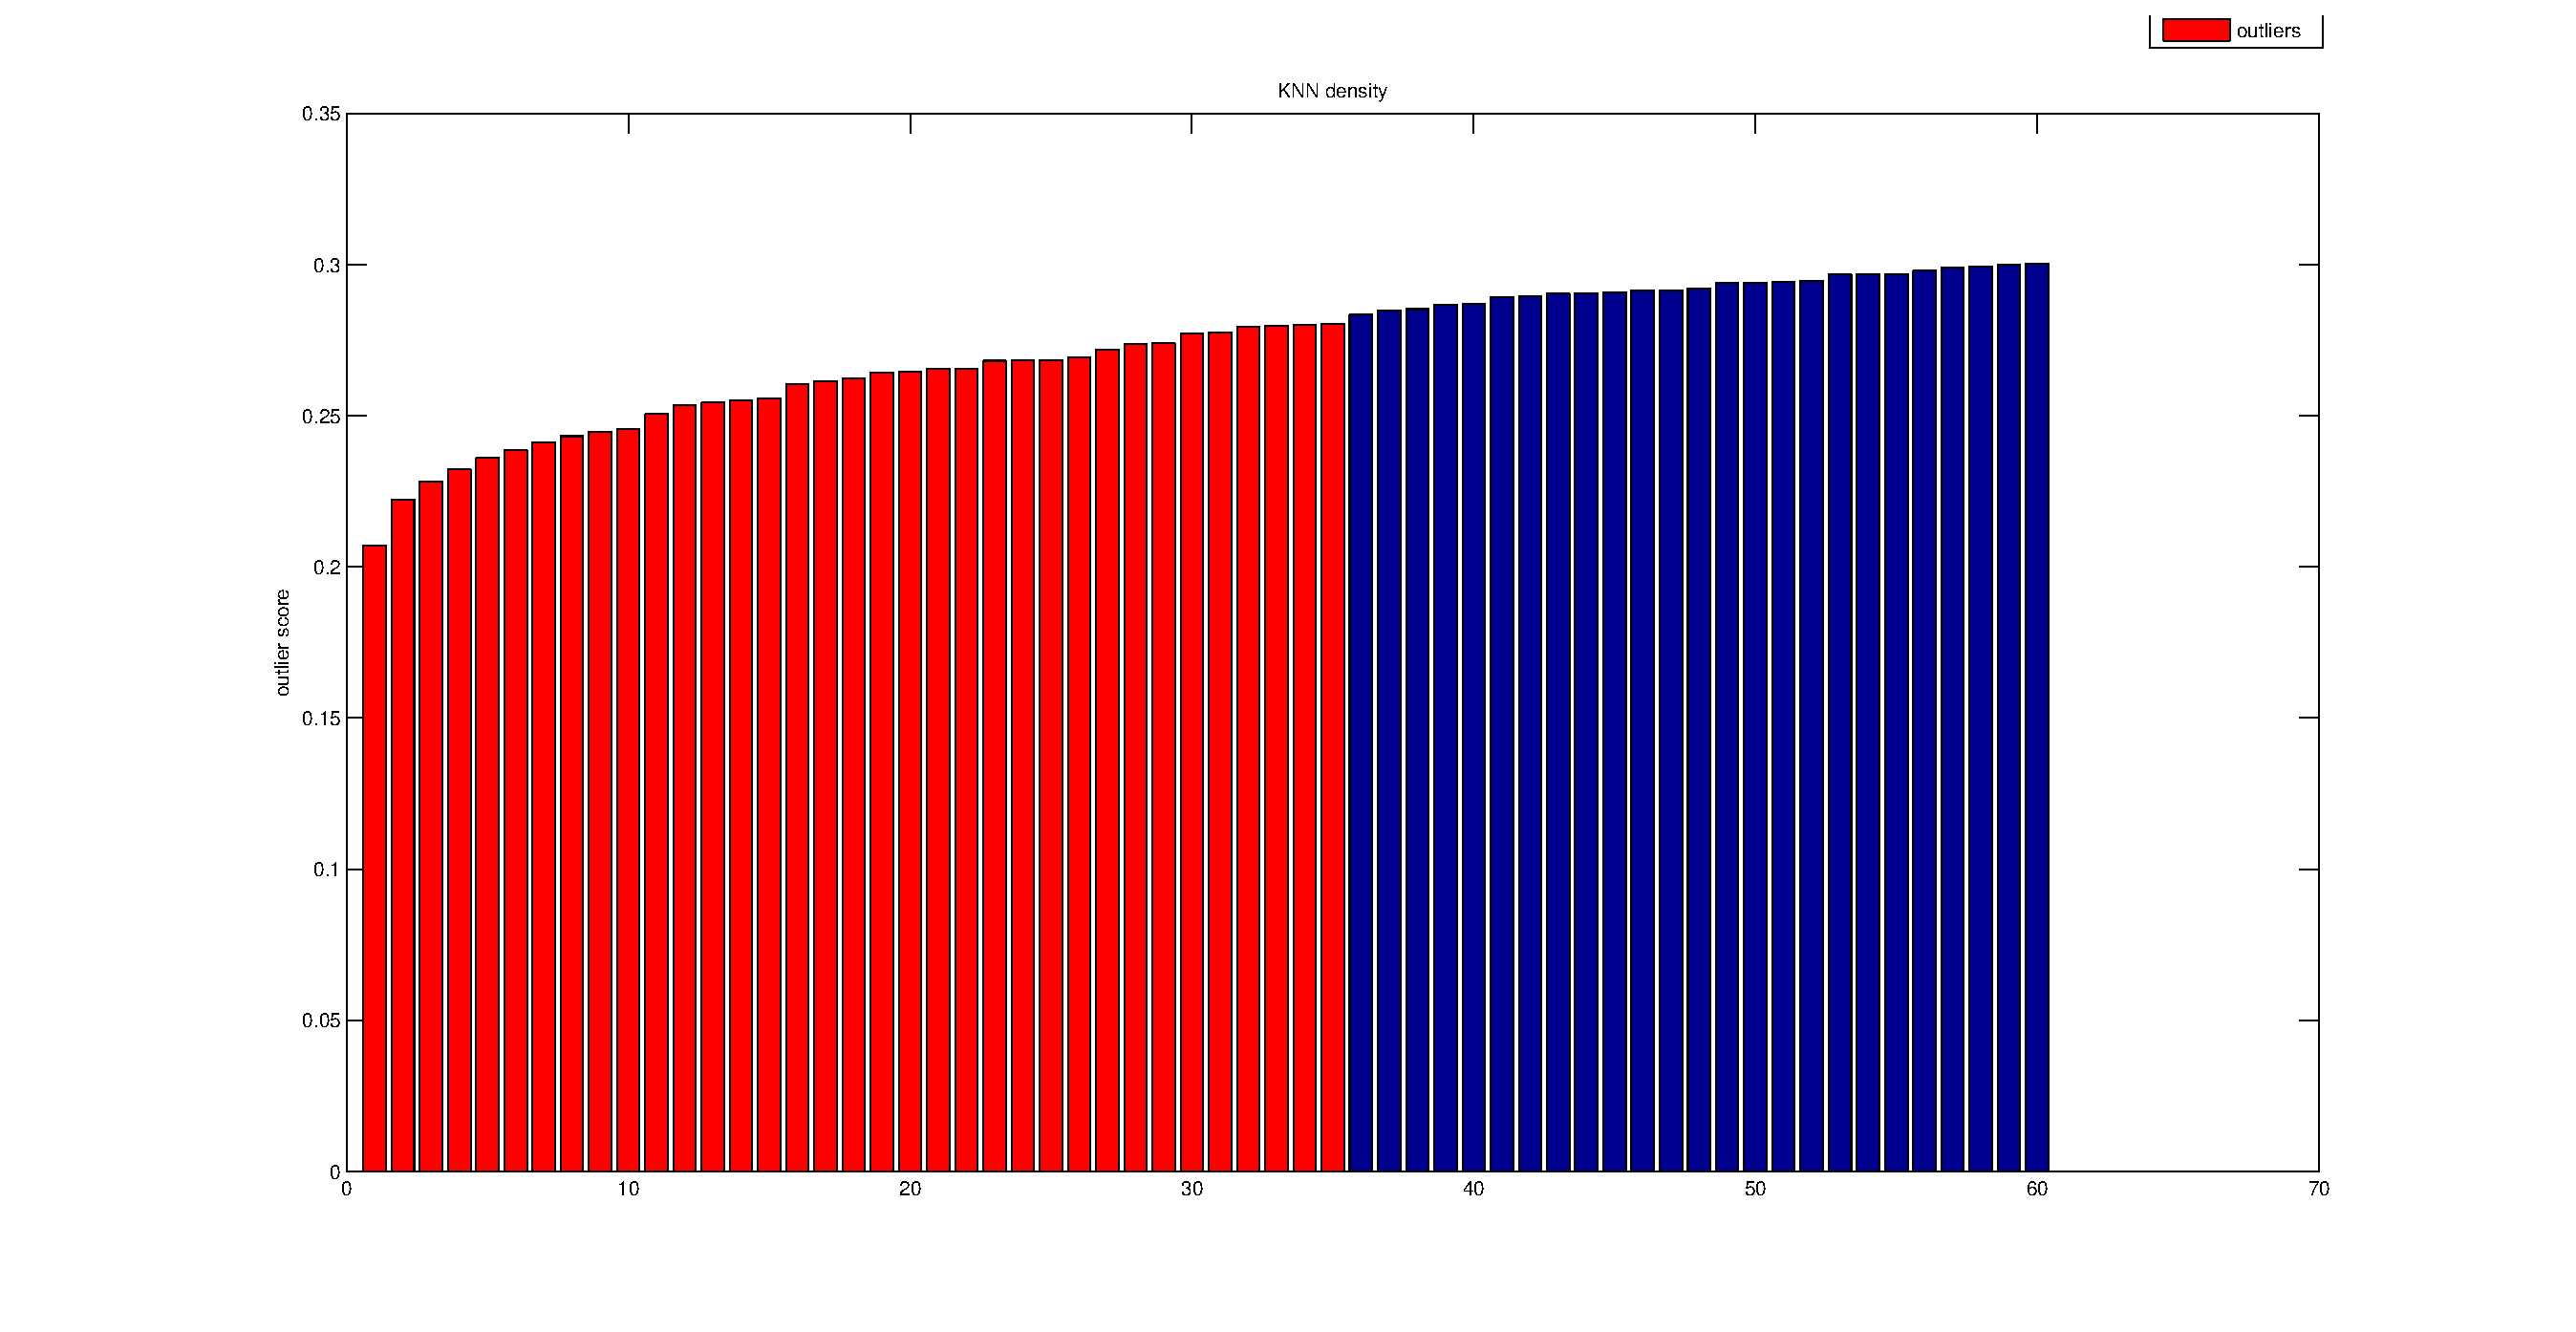
\includegraphics[width=7.4cm]{figures/02.eps}
                \caption{KNN density outliers}
         \end{subfigure} \\
	 \begin{subfigure}[b]{0.46\textwidth}
                 \linespread{1}
                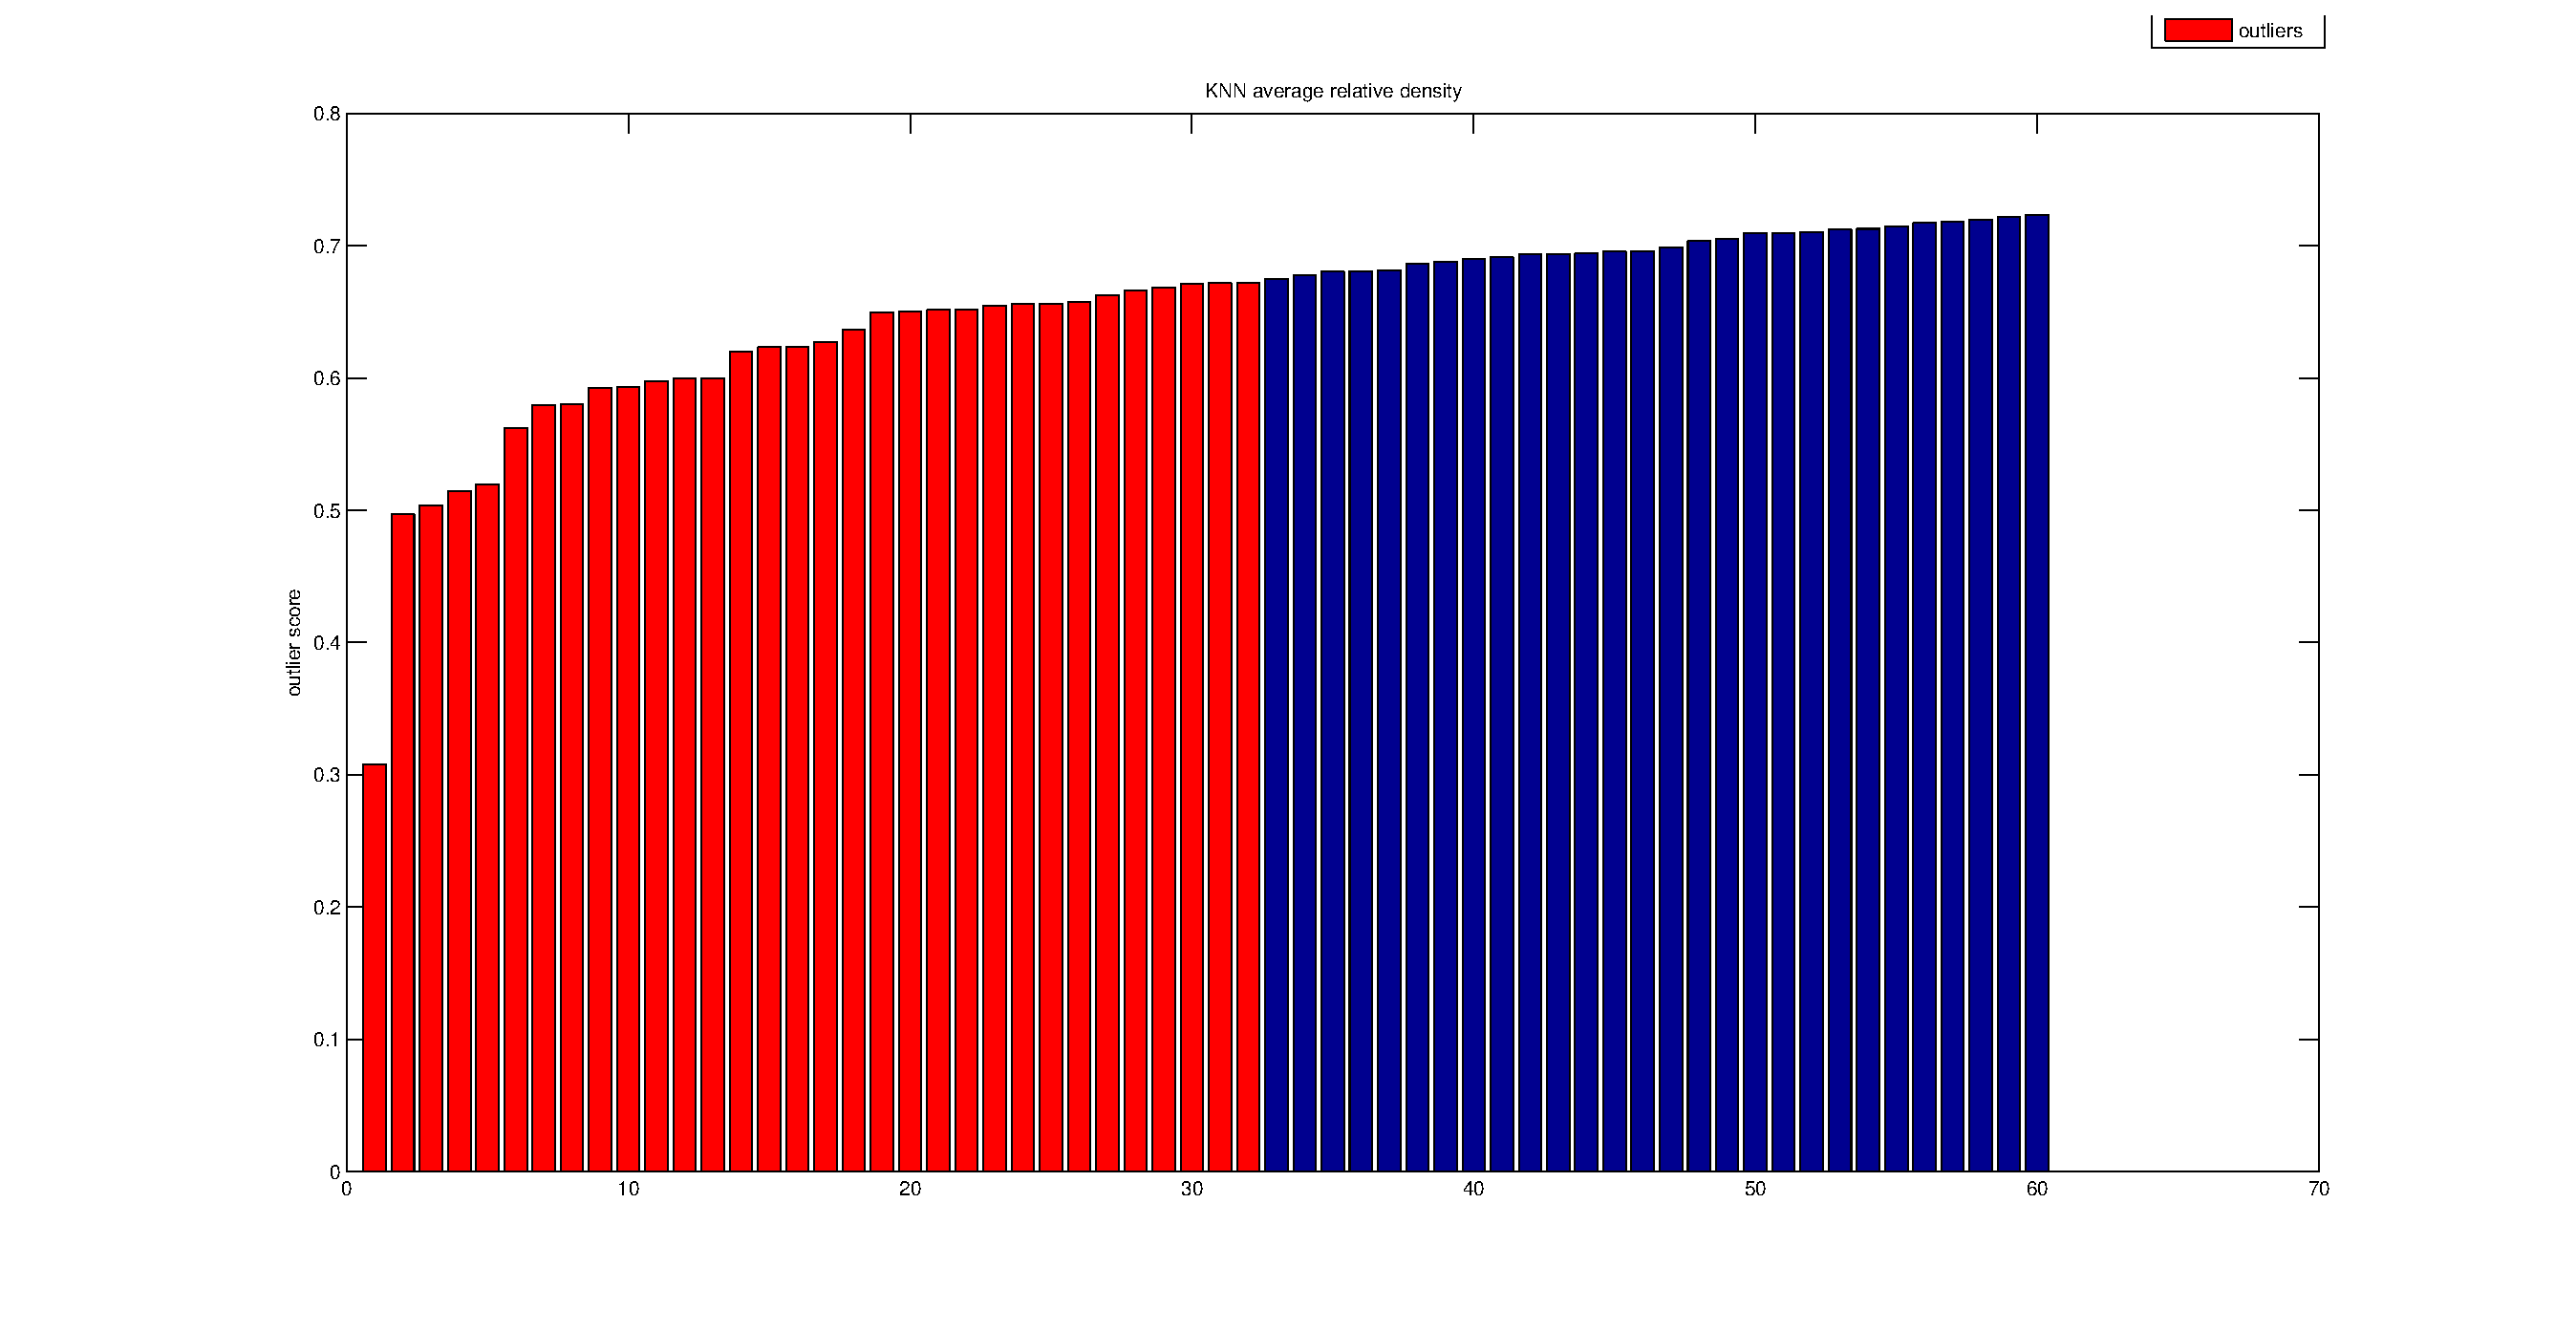
\includegraphics[width=7.4cm]{figures/03.eps}
                \caption{KNN avg rel. density outliers }
        \end{subfigure}
                \qquad
	\begin{subfigure}[b]{0.46\textwidth}
                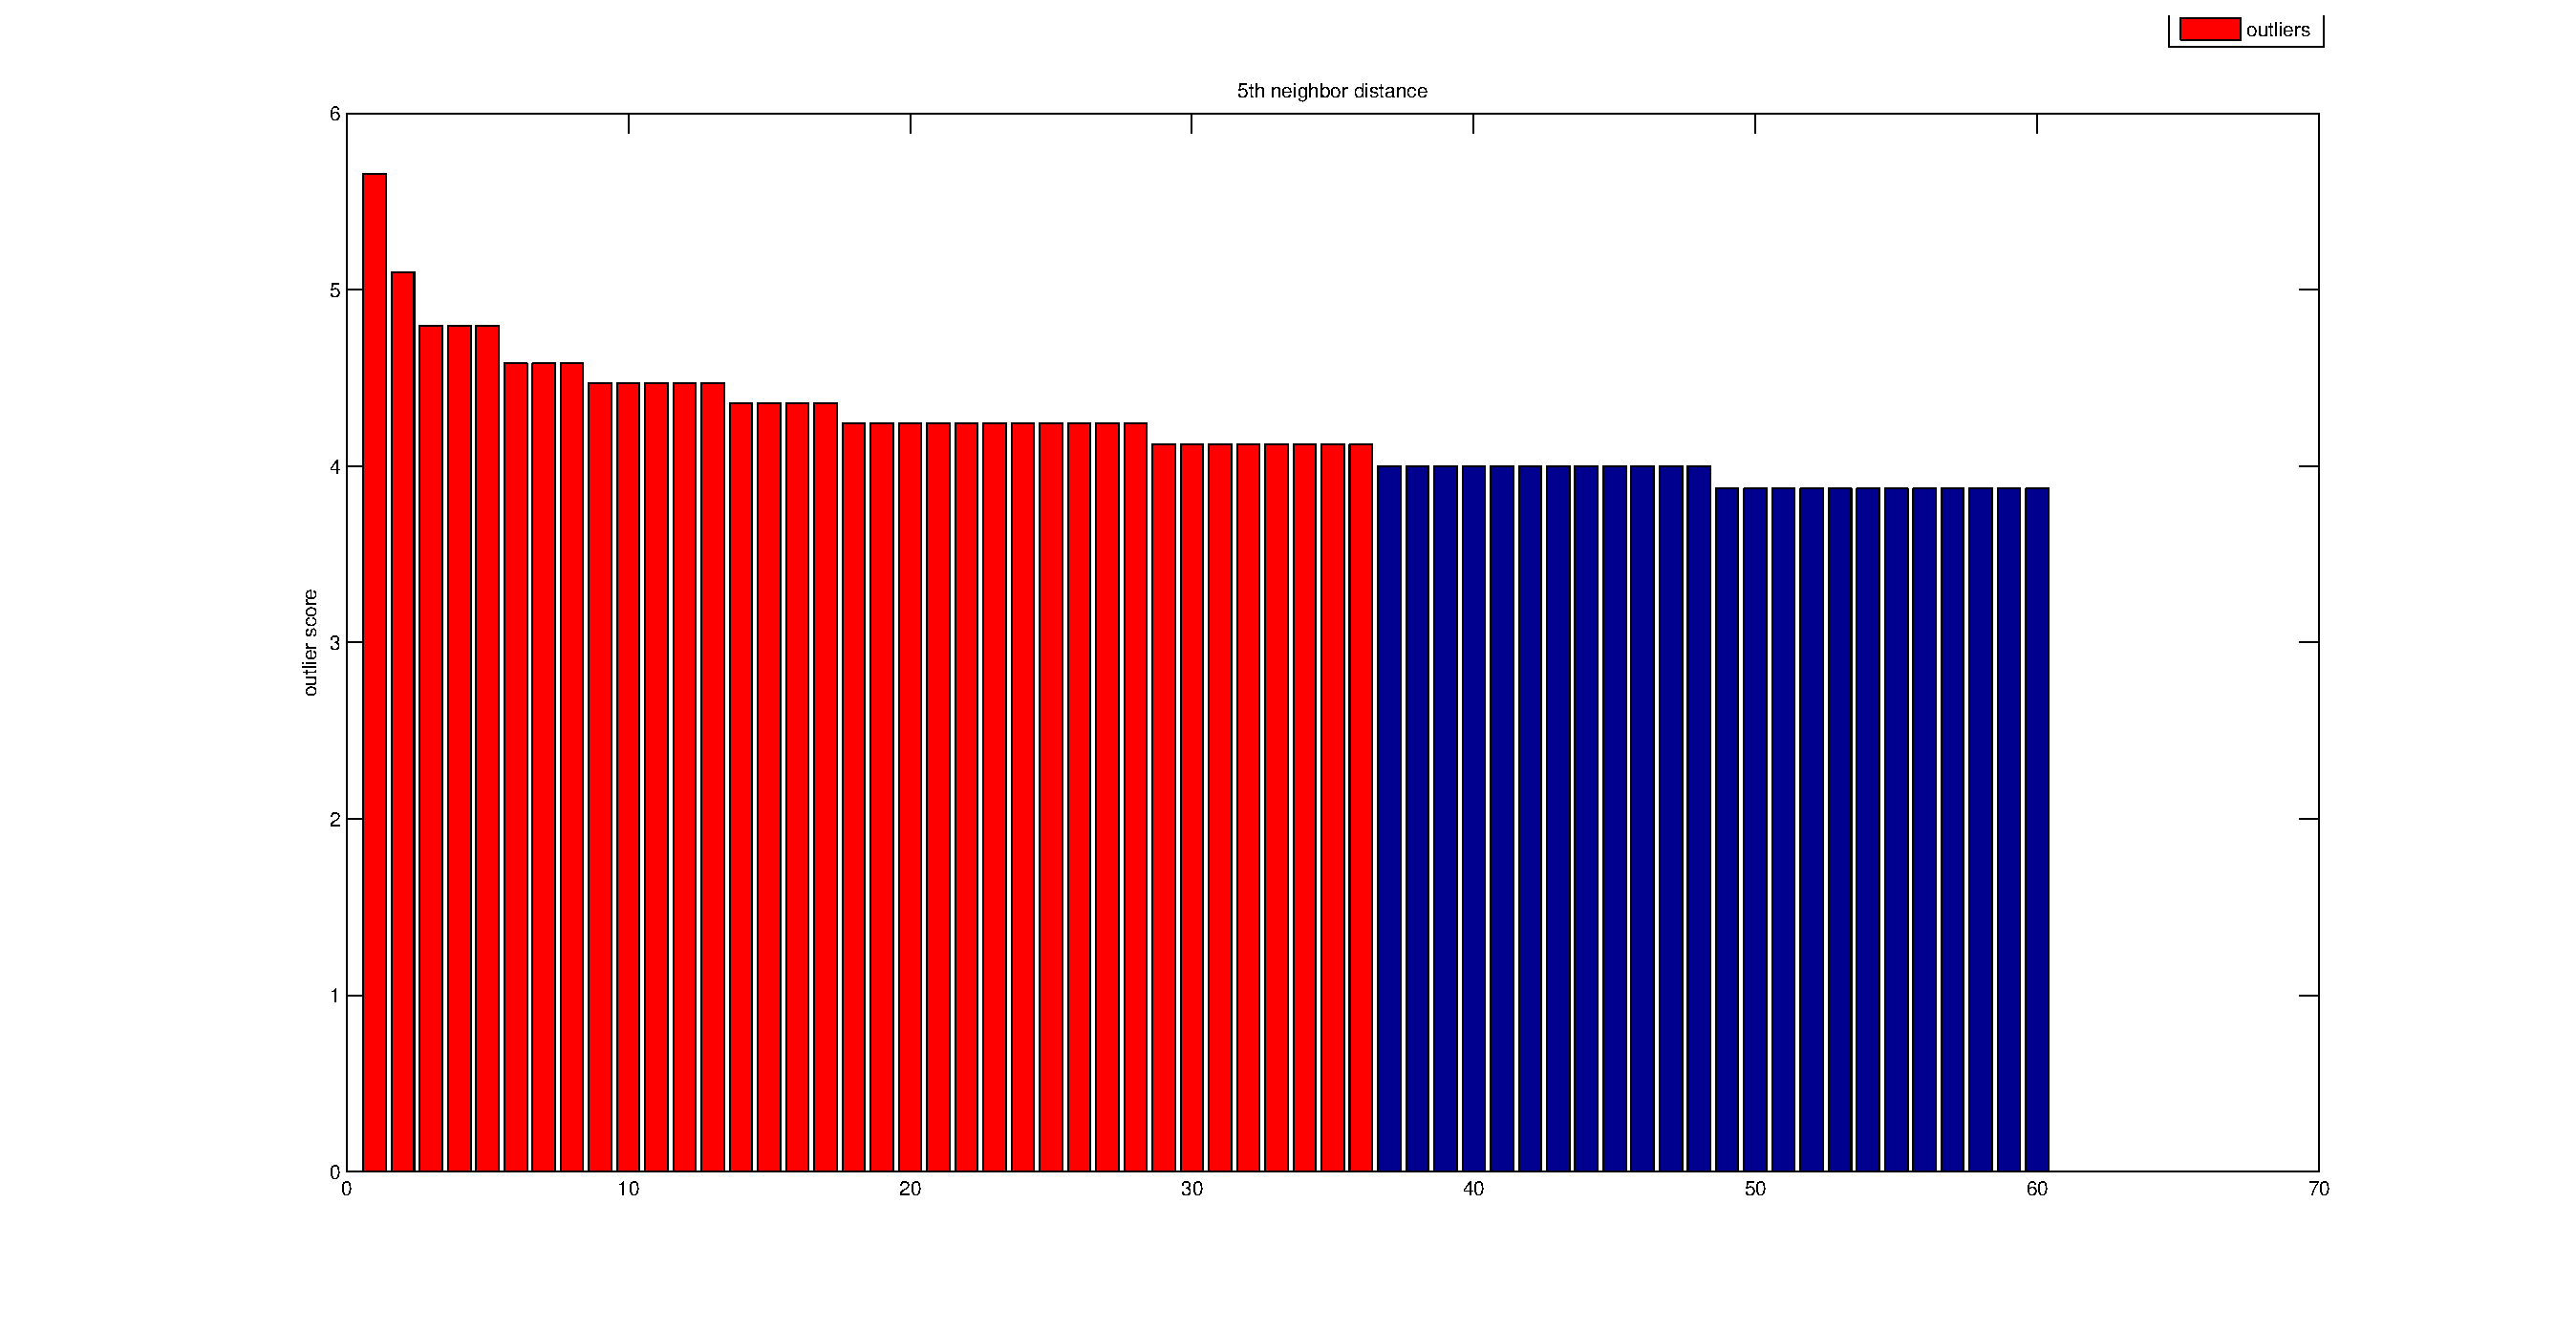
\includegraphics[width=7.4cm]{figures/04.eps}
                \caption{5th neighbor distance outliers}
         \end{subfigure} \\
        \caption{bar graph outliers}
         \label{fig:r1}
\end{figure}

To further understand the outliers distribution, for each scoring method we plot the outliers in the PCA space. Figures  \ref{fig:r2} shows that is not really possible to see a pattern for outliers in the PC1/PC2 space (maybe it could be possible find only few of them).
In figure \ref{fig:r3} you can see the outliers detected by all four methods.

\begin{figure}[htbp]
        \center
       	\begin{subfigure}[b]{0.55\textwidth}
                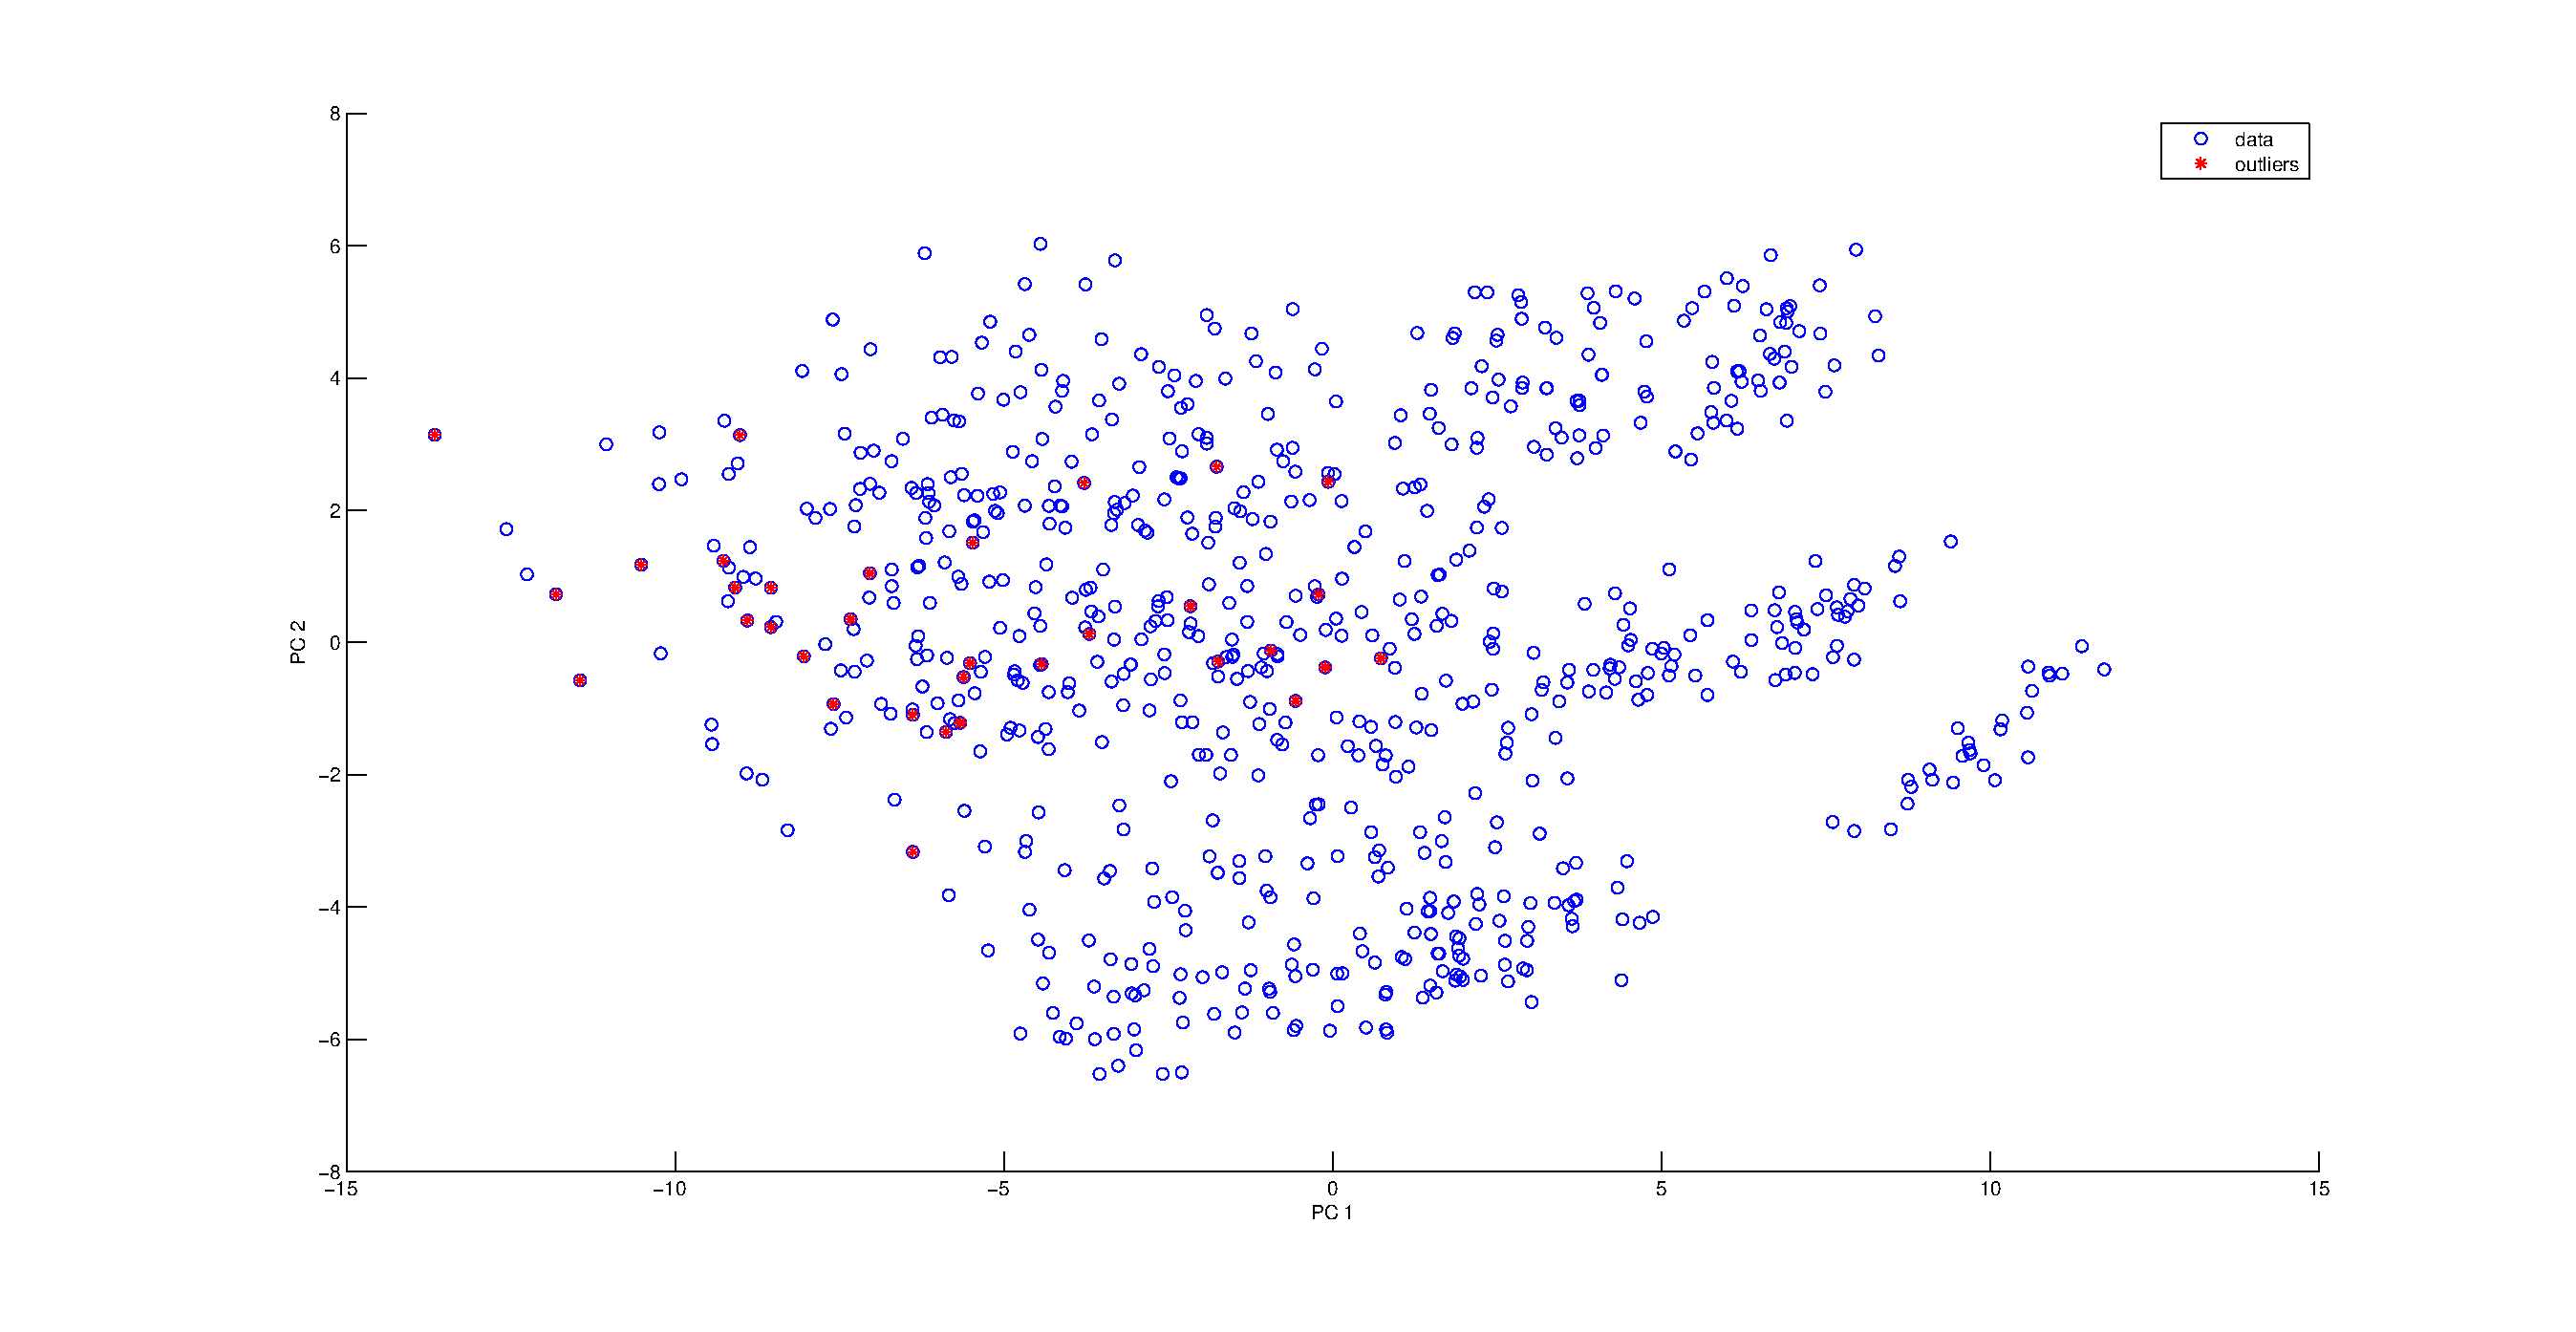
\includegraphics[width=10cm]{figures/pc1.eps}
                \caption{Density estimate outliers}
        \end{subfigure}%
        \quad
        \begin{subfigure}[b]{0.55\textwidth}
                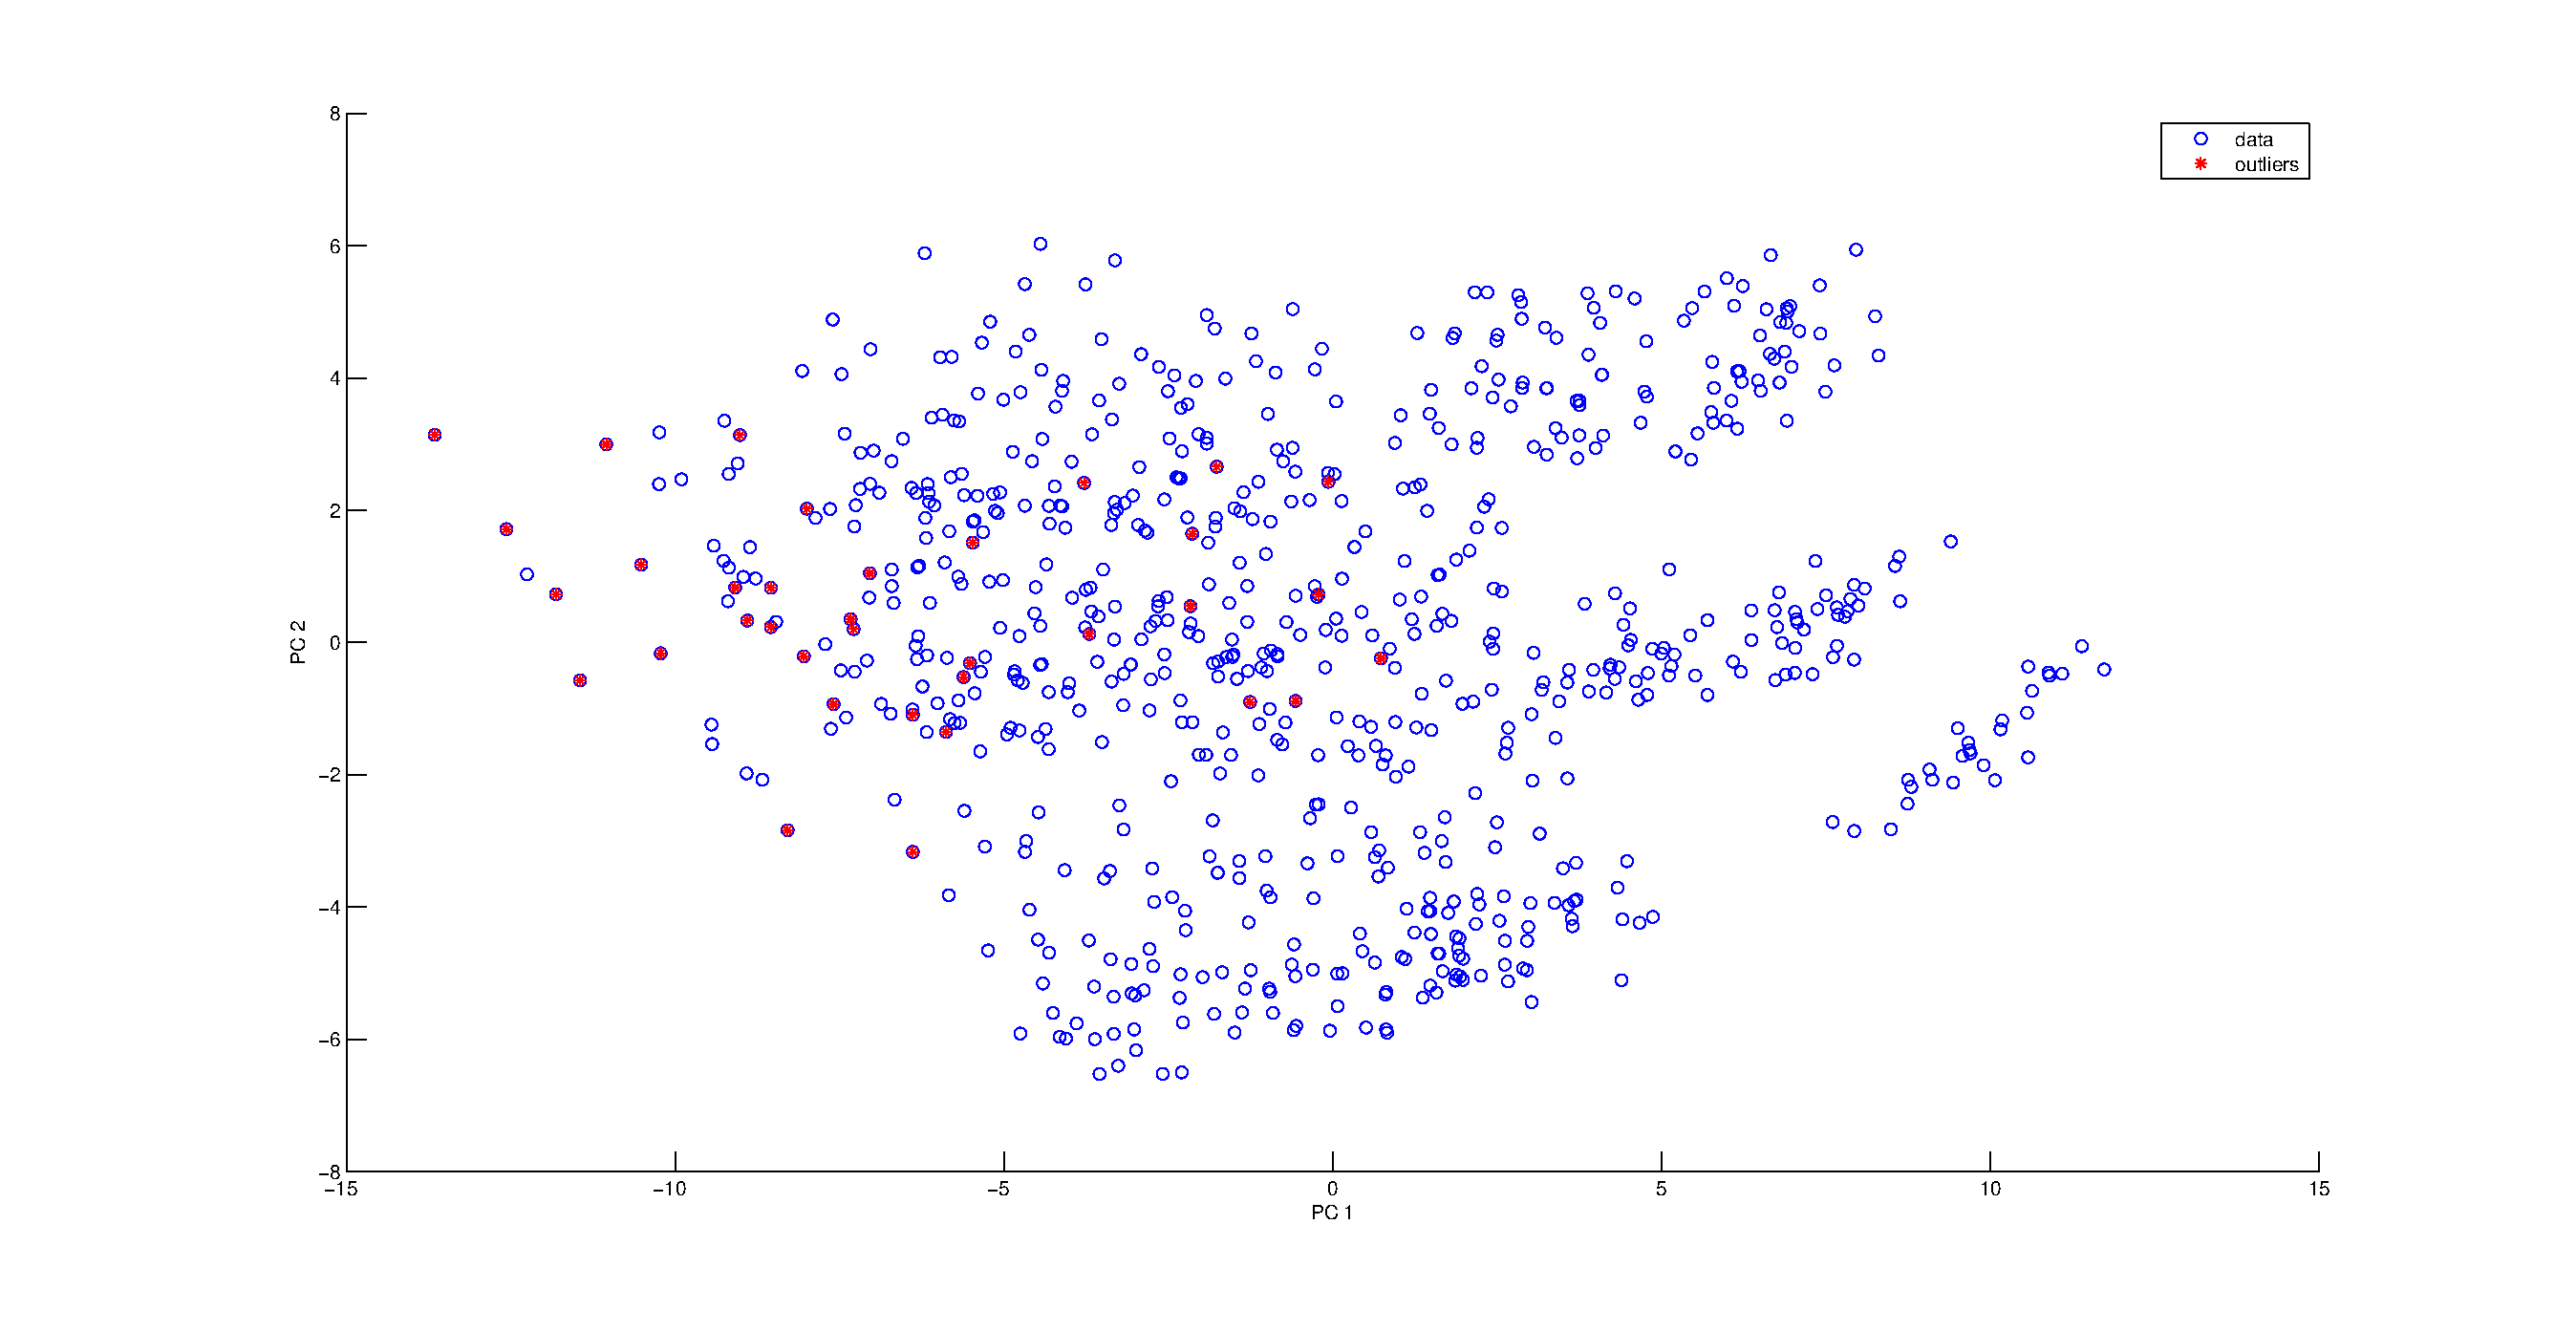
\includegraphics[width=10cm]{figures/pc2.eps}
                \caption{KNN density outliers}
         \end{subfigure} \\
	 \begin{subfigure}[b]{0.55\textwidth}
                 \linespread{1}
                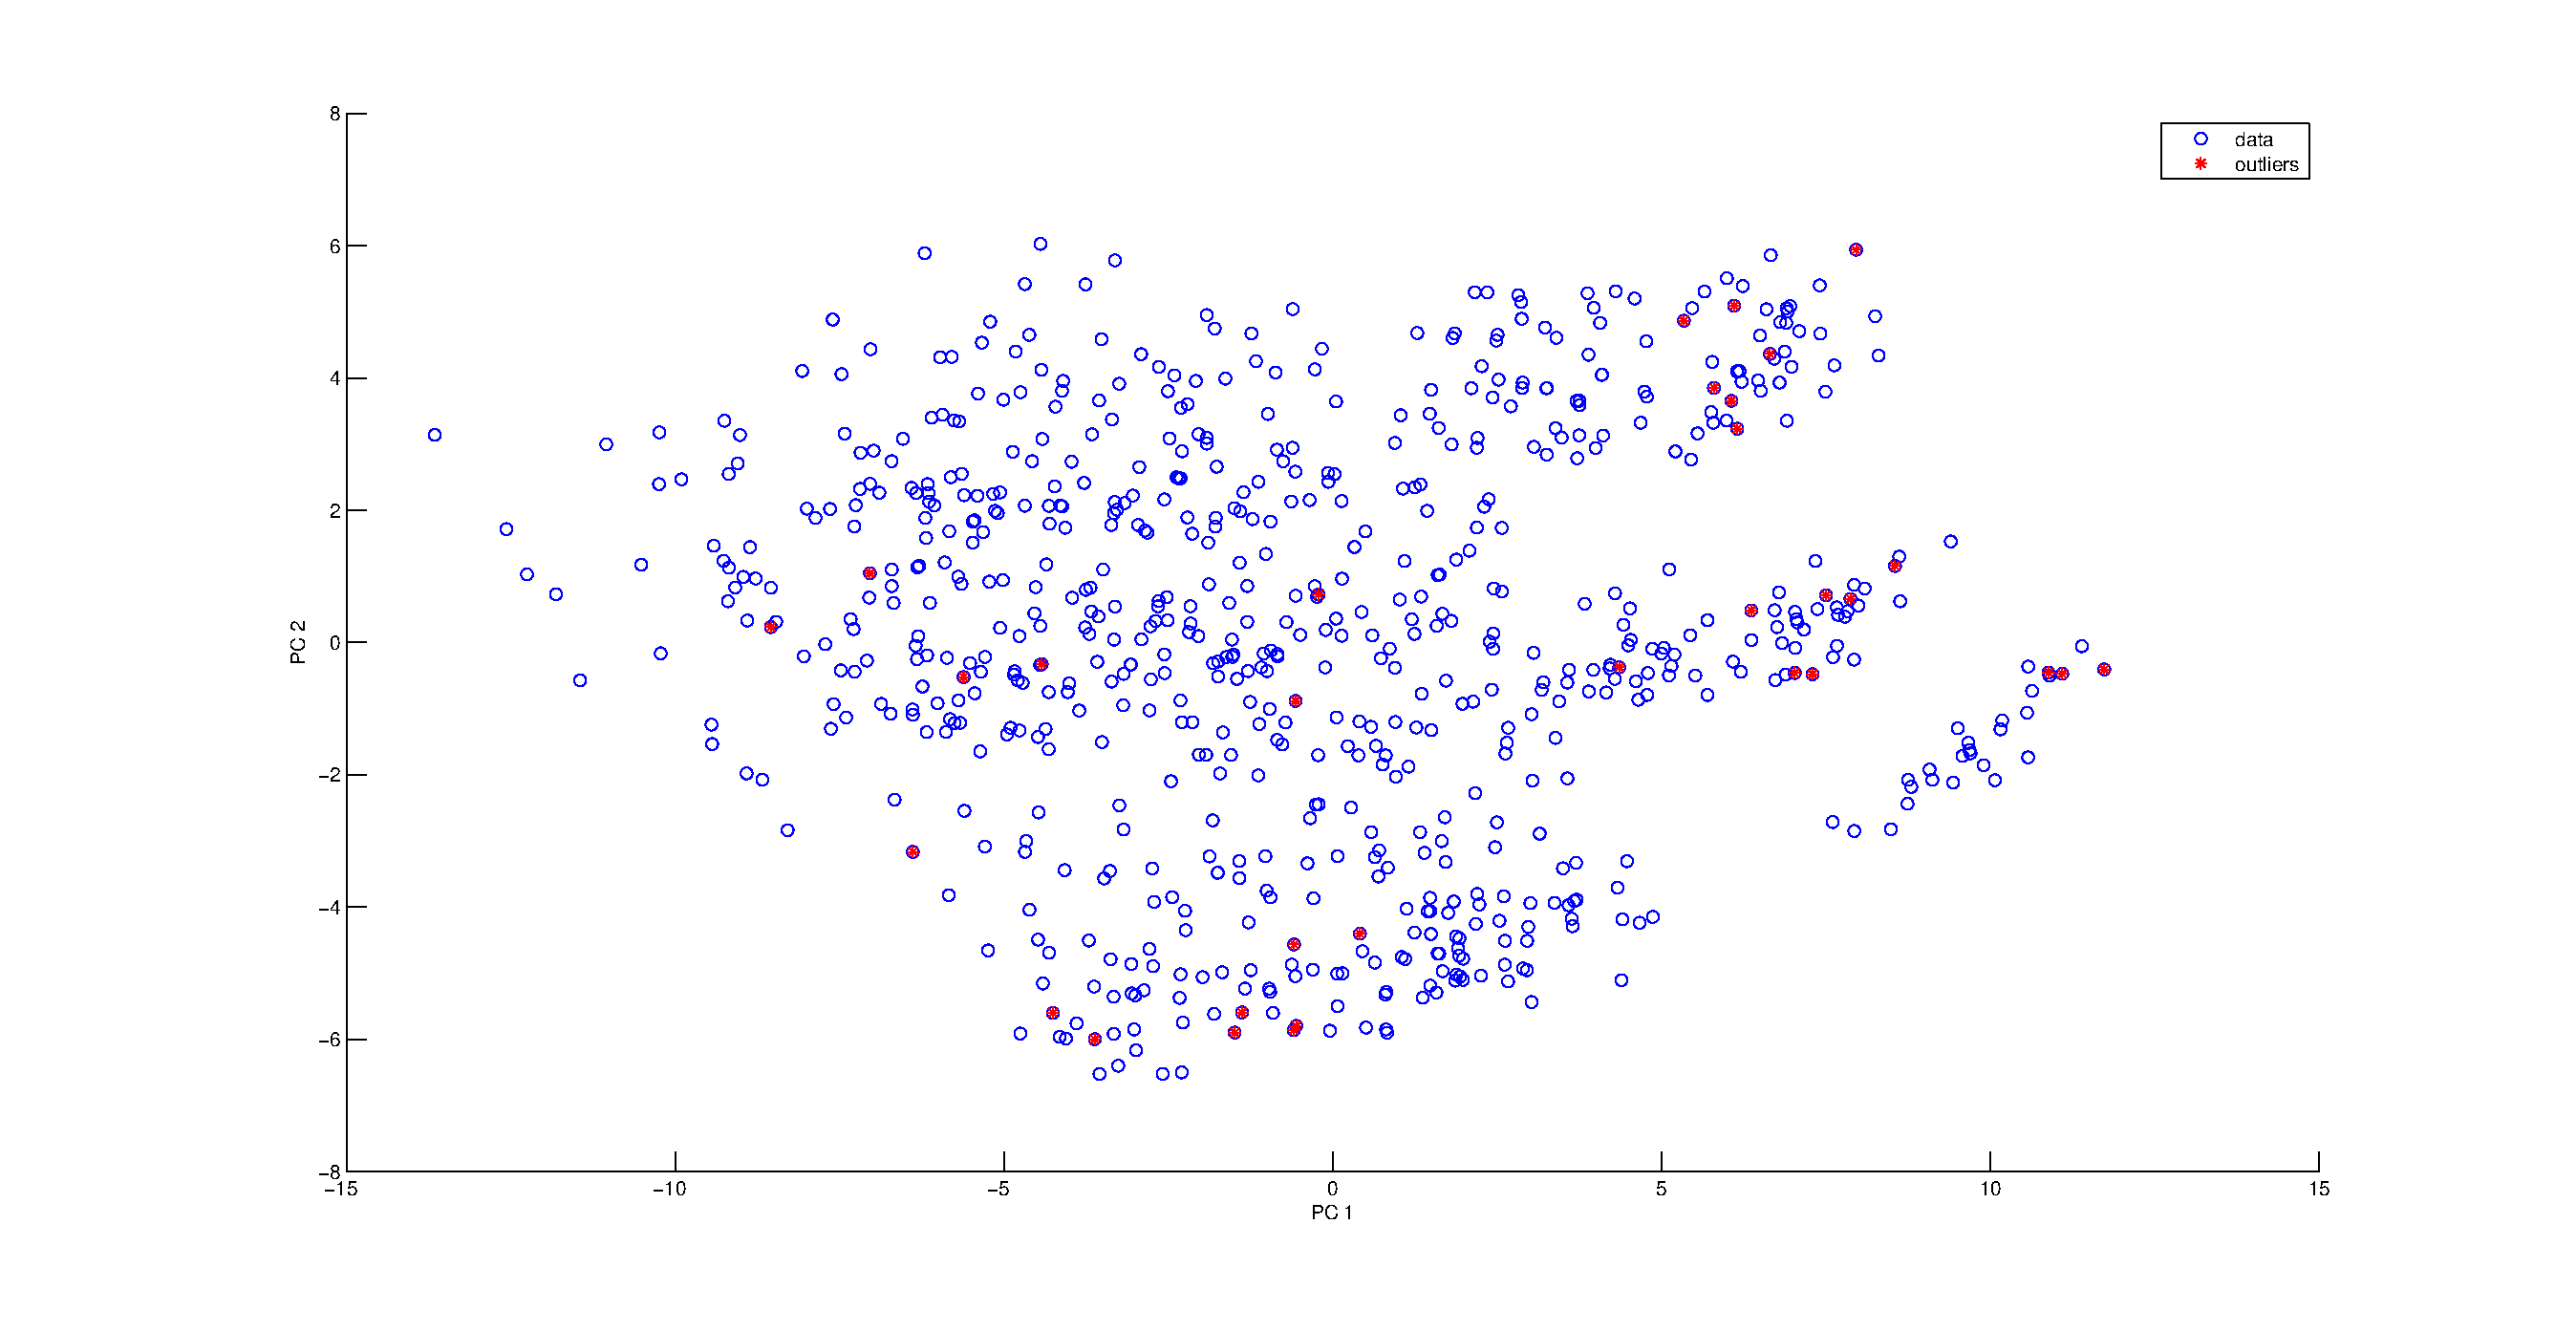
\includegraphics[width=10cm]{figures/pc3.eps}
                \caption{KNN average relative density outliers }
        \end{subfigure}
                \quad
	\begin{subfigure}[b]{0.55\textwidth}
                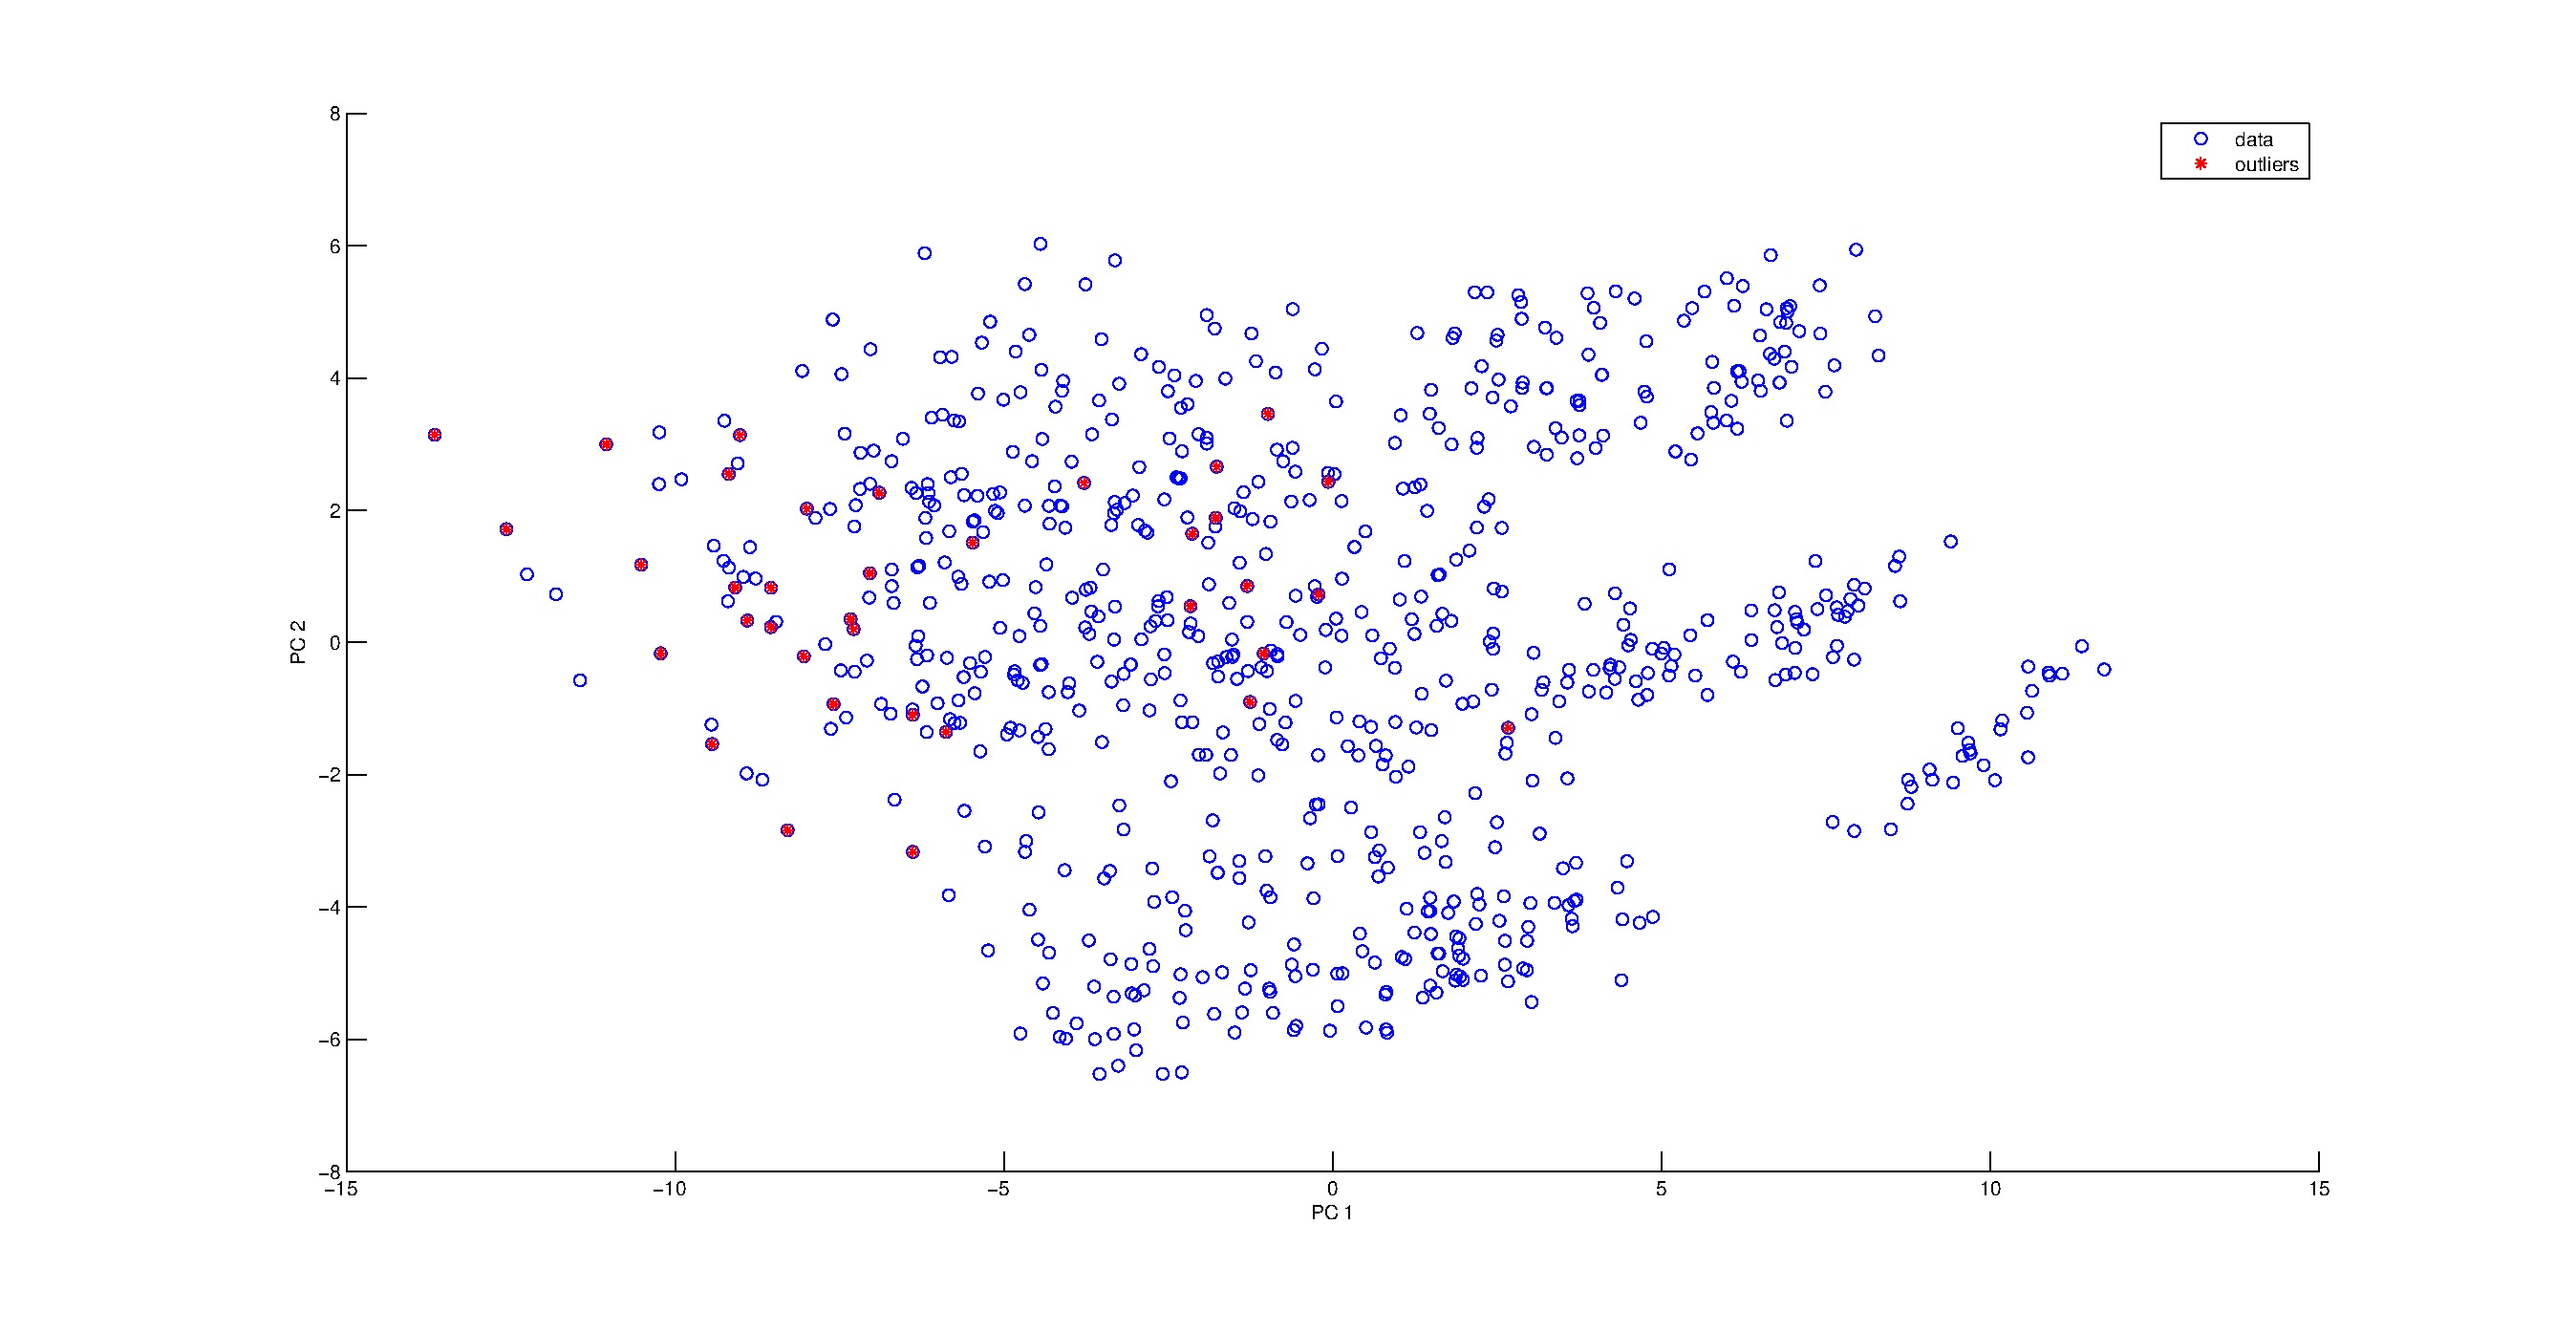
\includegraphics[width=10cm]{figures/pc4.eps}
                \caption{5th neighbor distance outliers}
         \end{subfigure} \\
        \caption{Principal component plot with outliers}
        \label{fig:r2}
\end{figure}

\begin{figure}[!tbh]
  \centering
  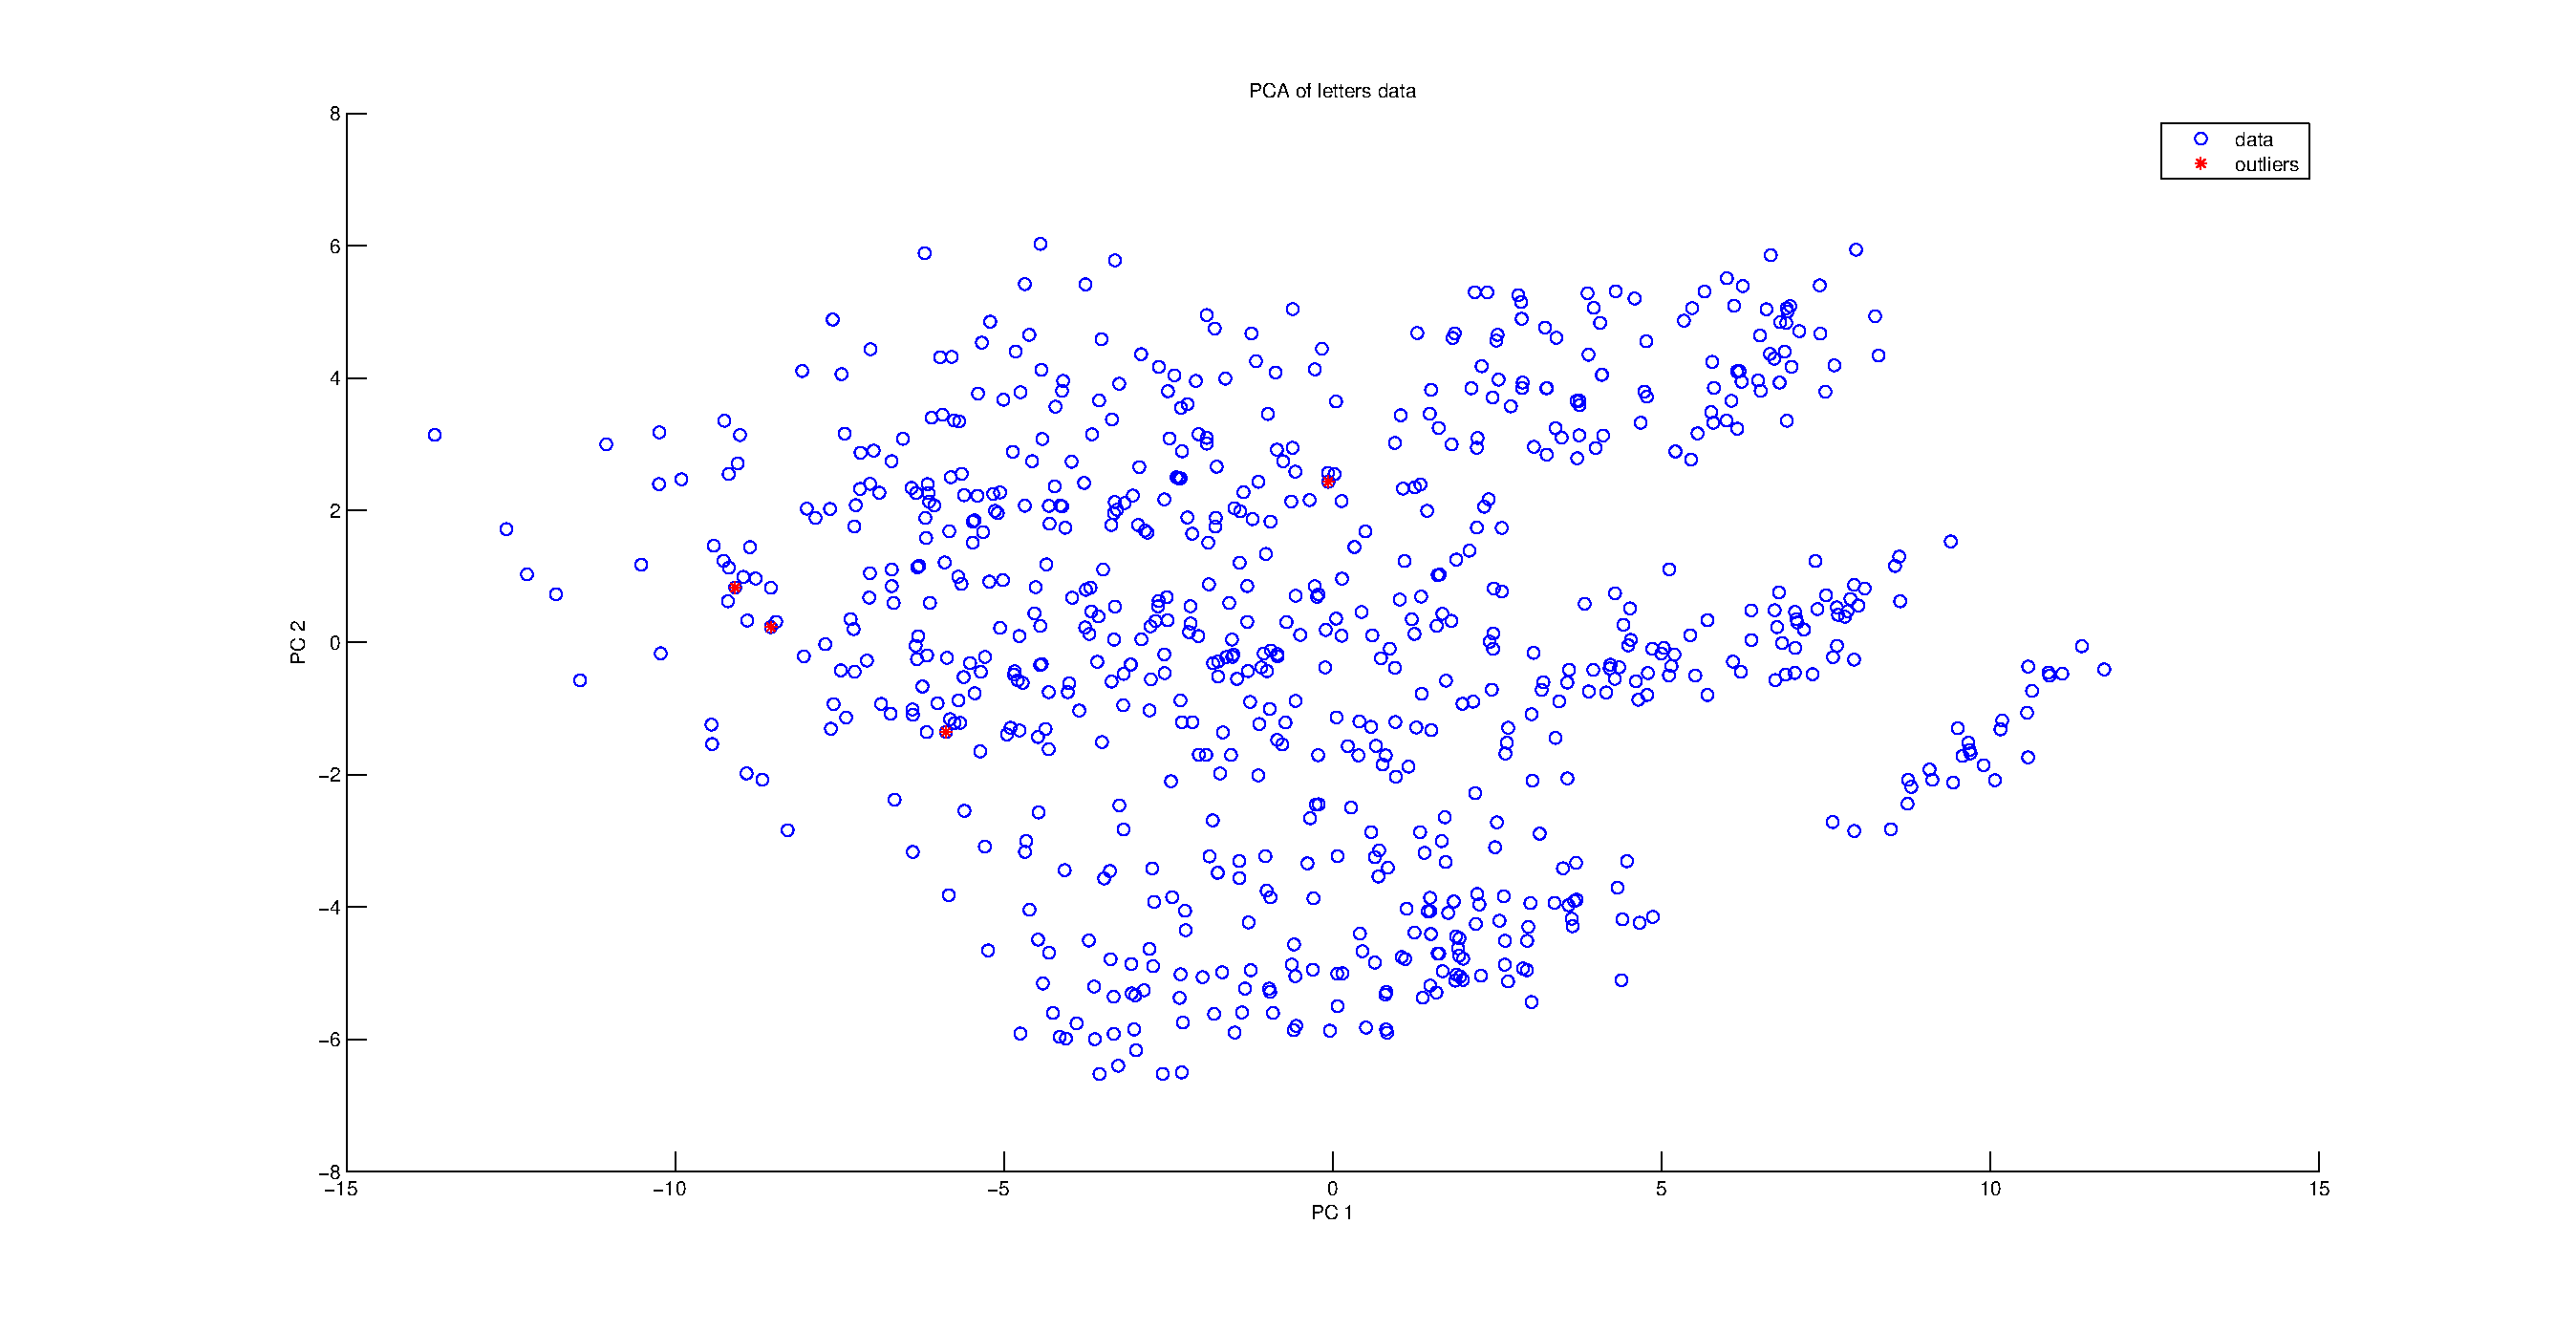
\includegraphics[width=1.0\textwidth]{figures/pc5}
  \caption{outliers detected by all four methods}
  \label{ffig:r3}
\end{figure}

We applied outlier detection using different metrics, and by setting an appropriate threshold we identified some outliers, constituting about 0.5\% of our dataset. Anyway we are never sure whether a certain pattern is an outlier but we can just suppose it especially because we have a wide dataset so is probable that some patterns are distant from other observations.
%\end{document}
